\documentclass[main.tex]{subfiles}
\begin{document}
\newpage
\section{Дополнительные материалы}

\begin{figure}[H]
	\centering
	\begin{subfigure}{.5\textwidth}
		\centering
		\includegraphics[width=\linewidth]{all/tsne/2d}
		\captionsetup{width=.8\linewidth}
		\caption{нефильтнованные данные на плоскости}
		\label{fig:all_tsne_2d}
	\end{subfigure}%
	\begin{subfigure}{.5\textwidth}
		\centering
		\includegraphics[width=\linewidth]{all/tsne/3d}
		\captionsetup{width=.8\linewidth}
		\caption{нефильтрованные данные в трёх измерениях}
		\label{fig:all_tsne_3d}
	\end{subfigure}

	\begin{subfigure}{.5\textwidth}
		\centering
		\includegraphics[width=\linewidth]{significant/tsne/2d}
		\captionsetup{width=.8\linewidth}
		\caption{данные с учётом только значимых полиморфизмов (на плоскости)}
		\label{fig:signif_tsne_2d}
	\end{subfigure}%
	\begin{subfigure}{.5\textwidth}
		\centering
		\includegraphics[width=\linewidth]{significant/tsne/3d}
		\captionsetup{width=.8\linewidth}
		\caption{данные только с учётом значимых полиморфизмов (в трёх измерениях)}
		\label{fig:signif_tsne_3d}
	\end{subfigure}
	\caption{Результат сокращения размерности с помощью t-SNE}
\end{figure}

\begin{figure}[H]
	\centering 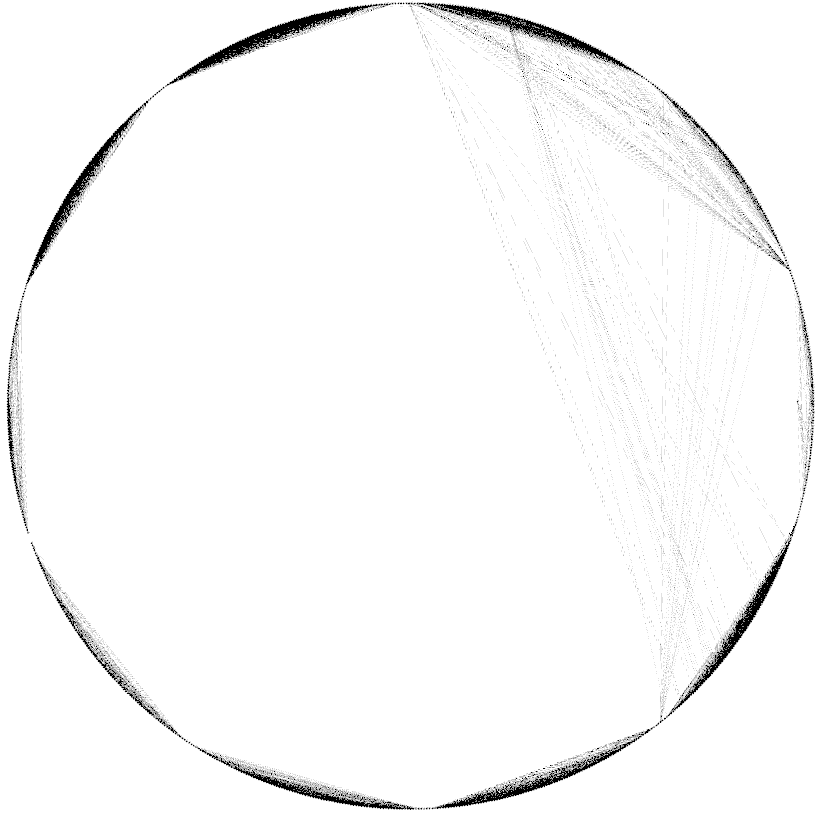
\includegraphics[width=\myPictWidth]{significant/manhattan/graph}
	\caption{Граф, построенный по матрице смежности (расстояние Хэмминга)}
	\label{fig:signif_manhattan_graph}
\end{figure}

\end{document}
